\documentclass[../main.tex]{subfiles}

\makeatletter
\@ifundefined{fromRoot}{%
  \newcommand{\fromRoot}[1]{../#1}
  
 % \usepackage{xr}
  % \externaldocument{../main}
}{}

\def\input@path{{\subfix{../}}}
%or: \def\input@path{{/path/to/folder/}{/path/to/other/folder/}}
\makeatother

\graphicspath{
  {\subfix{../}}
  {\subfix{./figures}}
  {\subfix{../figures}}
  {\subfix{./figures/logos-thesis/}}
  {\subfix{../figures/logos-thesis/}}
  {\subfix{./figures/rtexps-pics/}}
  {\subfix{../figures/rtexps-pics/}}
}

\hypersetup{
    pdfauthor   = {Camille MONIÈRE},
    pdftitle    = {Th\`{e}se (Présentation: implémentations)},
    pdfsubject  = {Th\`{e}se (Présentation: implémentations)},
%    pdfkeywords = {mots-cl\'{e}s},
}

\begin{document}

\section{Étude et exploitation du parallélisme}

\subsection{Rappel : Différents niveaux de parallélismes}

\begin{frame}{\acrfull{simd}}
  \begin{columns}
    \begin{column}{.5\linewidth}
      \centering
      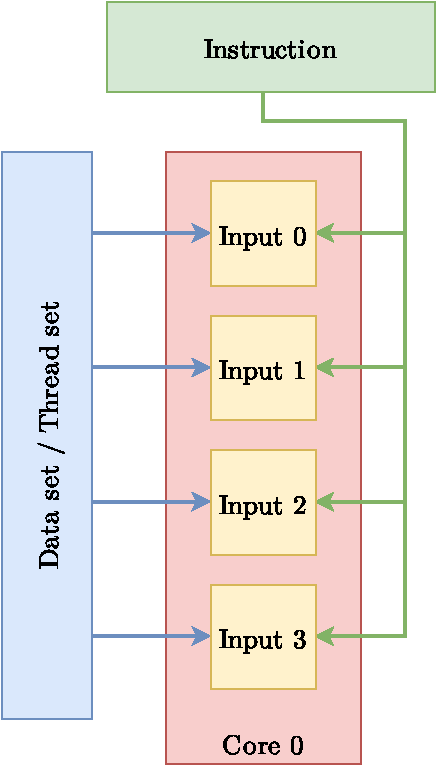
\includegraphics[
        width=\linewidth,
        height=.85\textheight,
        keepaspectratio=true
      ]{figures/drawiopdf/simd_simt.drawio.pdf}
    \end{column}
    \begin{column}{.5\linewidth}
      {}
      UC : Unité de Calcul
    \end{column}
  \end{columns}
\end{frame}

\begin{frame}{Single Process Multiple Data (SPMD)}
  \begin{columns}
    \begin{column}{.5\linewidth}
      \centering
      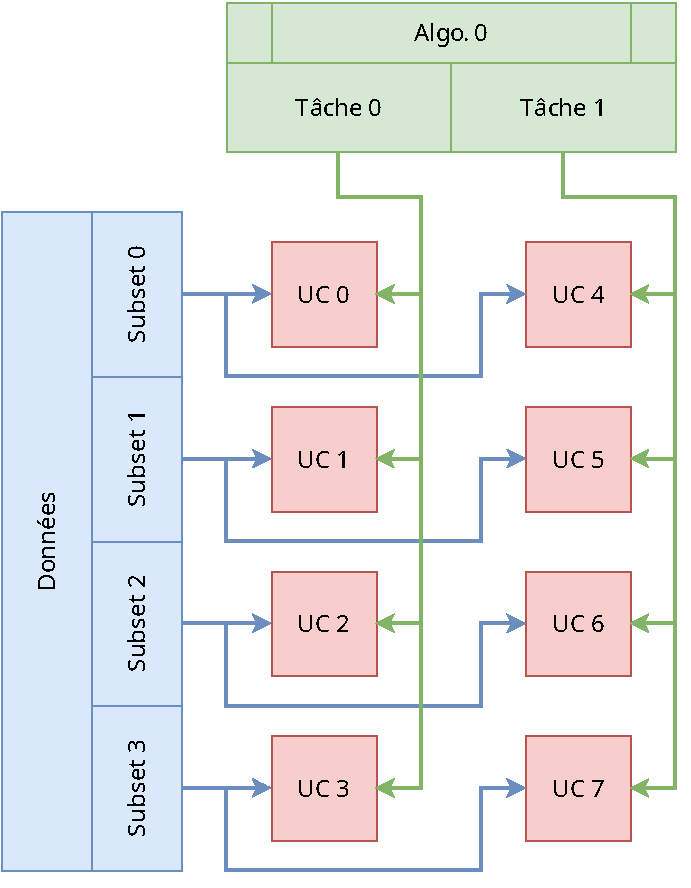
\includegraphics[
        width=\linewidth,
        height=.85\textheight,
        keepaspectratio=true
      ]{figures/drawiopdf/spmd.drawio.pdf}
    \end{column}
    \begin{column}{.5\linewidth}
      {}
      UC : Unité de Calcul
    \end{column}
  \end{columns}
\end{frame}

\begin{frame}{Multiple Processes Multiple Data (MPMD)}
  \begin{columns}
    \begin{column}{.5\linewidth}
      \centering
      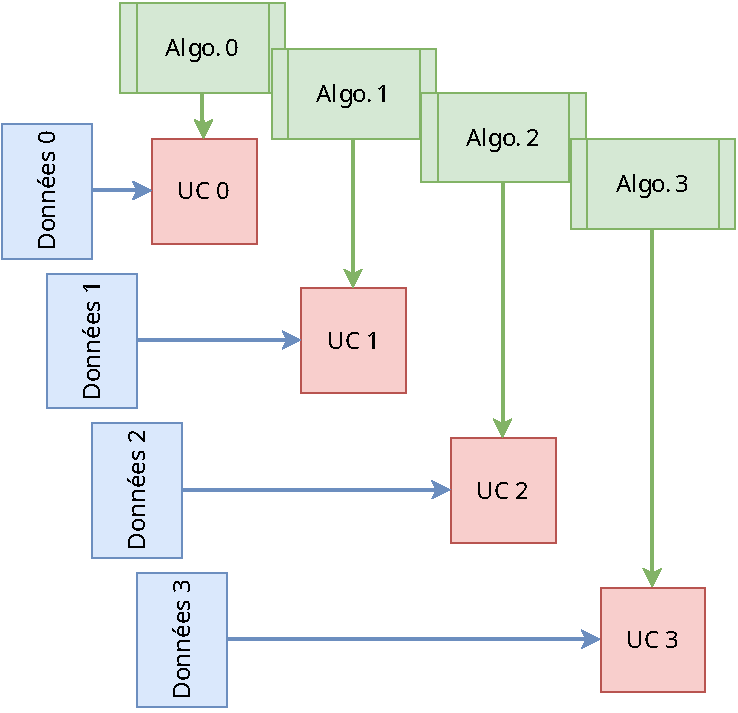
\includegraphics[
        width=\linewidth,
        height=.85\textheight,
        keepaspectratio=true
      ]{figures/drawiopdf/mpmd.drawio.pdf}
    \end{column}
    \begin{column}{.5\linewidth}
      {}
      UC : Unité de Calcul
    \end{column}
  \end{columns}
\end{frame}

\subsection{Étude du parallélisme}

\begin{frame}{\subsecname}
  \begin{center}
    \textcolor{RoyalBlue}{TODO}
  \end{center}
\end{frame}

\subsection{Les corrélations}

\begin{frame}{}
  \begin{center}
    \textcolor{RoyalBlue}{TODO}
  \end{center}
\end{frame}

\end{document}
